$A$ calls out a digit. Then $B$ places that digit into one of the empty cells, until all $8$ cells are filled by digits. $A$ wants to maximize the difference. $B$ tries to make it as small as possible. Prove that $B$ can place the digits so that the difference is at most $4000$. $A$ can call digits such that the difference is at least $4000$.
\begin{center}
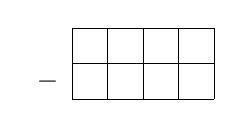
\begin{tikzpicture}[scale=0.45]
\draw (0,0) grid (4,2);
\node at (-0.7,0.5) {$-$};
\end{tikzpicture}
\end{center}
